%!TEX root=../../root.tex

\section{Lezione 2}
\subsection{Automi a stati finiti}
Prima di definire gli automi a stati finiti introduciamo alcuni concetti.
\begin{description}
	\item Un \emph{alfabeto} \`e un insieme $\Sigma$ che contiene dei simboli. Questi simboli possono essere lettere, cifre o rappresentazioni. Un esempio di alfabeto \`e quello binario $\Sigma_0 =$ $\{0, 1\}$.
	\item Una \emph{parola} \`e una sequenza di simboli che appartengono ad un certo alfabeto. Sia $x$ una parola indichiamo con $|x|$ la lunghezza della parola $x$. Esiste la \emph{parola vuota} e viene indicata con $\varepsilon$ e indica la parola di lunghezza $0$.
	\item $\Sigma^{\star}$ \`e l'insieme di tutte le parole che posso costruire con l'alfabeto $\Sigma$. $|\Sigma^{\star}| = \infty$
	\item Un \emph{linguaggio} $L$ \`e un sottoinsieme di $\Sigma^{\star}$.
\end{description}
Possiamo ora procedere con la definizione di automa a stati finiti. Spesso ci si riferisce ad essi con l'acronimo inglese DFA \emph{[Deterministic Finite state Automata]}. Un automa a stati finiti \`e una quintupla 
\[
	A = (Q, \Sigma, \delta, q_0. F)
\]
Dove:
\begin{description}
	\item $Q$ \`e un insieme finito di stati;
	\item $\Sigma$ \`e l'alfabeto di input;
	\item $q_0 \in Q$ \`e lo stato iniziale;
	\item $\delta : Q \times \Sigma \to Q$ \`e una funzione che dato uno stato di partenza e un simbolo in input restituisce lo stato di arrivo;
	\item $F \subseteq Q$ \`e l'insieme degli stati finali o di accettazione, ossia quegli stati che accettano parole in input.	 
\end{description}
Un automa a stati finiti pu\`o essere rappresentato attraverso un grafo dove i nodi rappresentano gli stati e sono etichettati con il nome dello stato. Gli stati sono il modo in cui un automa mantiene memoria di ci\`o che ha letto. Quando l'automa legge un simbolo $c$ in input trovandosi in un certo stato $q_1$ deve sapere in che stato transitare. Questa informazione \`e data funzione $\delta$, se tale stato \`e $q_2$ allora $\delta(q_1, c) = q_2$. Nel grafo questa informazione \`e rappresentata dagli archi che vengono etichettati dal simbolo che causa la transizione di stato. Al termine della lettura della parola l'automa si trover\`a in un certo stato $q_f$, se $q_f \in F$ allora si dice che la parola viene accettata dall'automa. In sostanza una parola \`e un cammino sul grafo degli stati. \\
Definiamo ora la funzione $\delta^{\star}$ che prende in input una parola $x$ e un qualsiasi stato $q \in Q$ e restituisce lo stato dell'automa al termine della computazione di $x$. Formalmente possiamo definire $\delta^{\star}$ ricorsivamente:
\[
     \delta^{\star} : Q \times \Sigma^{\star} \to Q
\]
\[
     \forall q \in Q, \delta^{\star}(q,\varepsilon) = q
\]
\[
     \forall q \in Q, \forall x \in \Sigma^{\star}, \forall a \in \Sigma, 
     \delta^{\star}(q,xa) = \delta (\delta^{\star}(q,x), a)
\]
Sia $A$ un certo automa, $L(A)$ \`e il linguaggio di $A$, ossia l'insieme delle parole accettate da A. Pi\`u formalmente lo possiamo definire come segue: 
\[
    L(A) = \{ x | x \in \Sigma^{\star} \land \delta^{\star}(q_0,x) \in F \}
\]
Allo stesso modo si pu\`o definire $L(A)^c$, ossia l'insieme delle parole non accettate dall'automa $A$.

\subsection{Classe dei linguaggi regolari}
Possiamo riunire sotto la classe dei linguaggi regolari tutti i linguaggi per cui esiste un automa che accetta quel linguaggio. Formalmente:
\[
     REG = \{ L | L \subseteq \Sigma^{\star} \exists A \in DFA \land L(A) = L \}
\]
\paragraph{Ordine canonico} Indichiamo con \emph{ordine canonico} un ordinamento quasi lessicografico. Pi\`u formalmente possiamo definirlo come segue: \newline
Siano $x$, $y$ parole, $x < y \Leftrightarrow |x| < |y| \lor  |x| = |y|$ e x precede y in ordine lessicografico.\newline
Prendendo come esempio $\leftidx{\Sigma}{_0^{\star}}$ notiamo che l'ordinamento canonico \`e: 
\[
	\varepsilon, 0, 1, 00, 01, 10, 11, 000, 001, 010, 011, 100, 101, 110, 111 ...
\]
Dimostriamo ora che $\leftidx{\Sigma}{_0^{\star}}$ \`e un insieme numerabile, per far ci\`o costruiamo una biezione da $\mathbb{N}$ a $\leftidx{\Sigma}{_0^{\star}}$. \newline
Sia $f :  \mathbb{N} \to \leftidx{\Sigma}{_0^{\star}}$, 
\begin{description}
	\item $f(2^n) = 0^n$ 
	\item $f(2^n + i) = bin_n(i)$ $1 \geq i \leq 2^n-1$
\end{description}
Per $0^n$ si intende la parola formata da tutti $0$ lunga n.\newline
Per $bin_n(i)$ si intende la parola che corrisponde alla rappresentazione in binario di $i$ lunga $n$.\newline
\begin{tabular}{|l|l|l|l|l|l|l|l|l|l|l|l|l|l|l|l|}
\hline
$\varepsilon$ & 0 & 1 & 00 & 01 & 10 & 11 & 000 & 001 & 010 & 011 & 100 & 101\\
\hline
$2^0$ & $2^1$ & $2^1+1$ & $2^2$ & $2^2+1$ & $2^2+2$ & $2^2+3$ & $2^3$ & $2^3+1$ & $2^3+2$ & $2^3+3$ & $2^3+4$ & $2^3+5$\\
\hline
1 & 2 & 3 & 4 & 5 & 6 & 7 & 8 & 9 & 10 & 11 & 12 & 13\\
\hline
\end{tabular}
\newline
--manca dimostrazione biezione--
\paragraph{Unione di linguaggi regolari}
Vogliamo determinare se l'operazione di unione di linguaggi regolari \`e chiusa in $REG$, pi\`u formalmente ci stiamo chiedendo:
\[
    L, L' \in REG \Rightarrow L \cup L' \in REG
\]
La risposta \`e s\`i, e rappresenta il primo passo nella costruzione di automi sempre pi\`u complessi.
\newline
\emph{Dimostrazione:} Se $L \in REG$ allora $\exists A_1$ tale che $L(A_1) = L$, lo stesso vale per $L'$, quindi $\exists A_2$ tale che $L(A_2) = L'$. Supponiamo di costruire un terzo automa $A_3$ che contenga sia $A_1$ che $A_2$ e che valuti l'input contemporaneamente sia su $A_1$ che su $A_2$ e accetti la parola solo se  \`e accettata almeno da uno dei due.
\newline
Il seguente esempio render\`a tutto pi\`u chiaro: \newline
$L = \{x | x \in \{a,b\}^{\star}$ e con un numero pari di $a \}$ \newline
$L' = \{x | x \in \{a,b\}^{\star} \land x=ybz \land y,z \in \{a,b\}^{\star} \}$ ossia l'insieme delle parole in $\{a,b\}^{\star}$ che hanno almeno una b. \newline
Costruiamo gli automi $A_1$ t.c. $L(A_1) = L$ e $A_2$ t.c. $L(A_2) = L'$. 
\begin{figure}[H]
    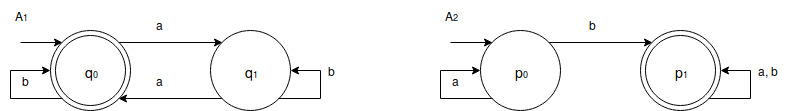
\includegraphics[width=1\textwidth]{a1a2}
\end{figure}
Ora costruiamo l'\emph{automa prodotto} rappresentando tutte le possibili combinazioni di stati che i due automi possono assumere in qualsiasi istante. Lo stato iniziale  \`e lo stato che ha come combinazione gli stati iniziali degli automi di partenza.\newline
Per capire come aggiungere gli archi consideriamo lo stato $(q_0, p_0)$, iniziamo chiedendoci in che stato l'automa deve transitare se l'input \`e $a$. \newline
$\delta_3((q_0, p_0),a)=(\delta_1(q_0,a),\delta_2(p_0,a))=(q_1,p_0)$, quindi aggiungiamo l'arco etichettato $a$ da $(q_0, p_0)$ a $(q_1,p_0)$. Con la stessa logica aggiungiamo tutti gli archi e otteniamo il seguente automa.\newline
Ora dobbiamo decidere quali sono gli stati finali. Dato che vogliamo ottenere l'unione dei due linguaggi gli stati finali sono quelli che nella propria etichetta contengono almeno uno stato finale degli automi di partenza.
\begin{figure}[H]
  \centering
    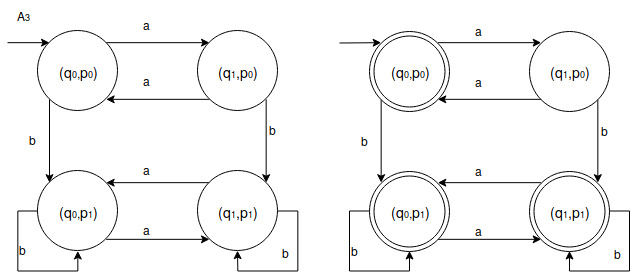
\includegraphics[width=1\textwidth]{a3}
\end{figure}
